\documentclass{article}
\usepackage[preprint]{neurips_2026}

\usepackage[utf8]{inputenc}
\usepackage[T1]{fontenc}
\usepackage{hyperref}
\usepackage{url}
\usepackage{booktabs}
\usepackage{amsfonts}
\usepackage{amsmath}
\usepackage{microtype}
\usepackage{xcolor}
\usepackage{graphicx}
\hypersetup{hidelinks}

% This is an ES 678 course paper, not a conference submission.
\makeatletter
\renewcommand{\@noticestring}{ES 678 Course Project}
\makeatother

% Auto-generated by src/paper_numbers.py from results/ and history/; do not edit by hand.
\newcommand{\Ndupnames}{42}
\newcommand{\Nmajshare}{19.1}
\newcommand{\Nmajlabel}{Laying}
\newcommand{\Nsdmin}{0.04}
\newcommand{\Nsdmax}{0.75}
\newcommand{\Nngrav}{60}
\newcommand{\Nnkeep}{501}
\newcommand{\Nnlinks}{6,752}
\newcommand{\Nnpairs}{7,351}
\newcommand{\Nnseg}{600}
\newcommand{\Nseglenmed}{12}
\newcommand{\Nseglenmax}{29}
\newcommand{\Nsegperminsa}{4}
\newcommand{\Nsegpermedsa}{4}
\newcommand{\Nnseeds}{10}
\newcommand{\Nrfgaplargest}{10}
\newcommand{\NoverlapR}{93.6}
\newcommand{\NsaS}{99.4}
\newcommand{\Ngrpvalsubjmin}{4}
\newcommand{\Ngrpvalsubjmax}{5}
\newcommand{\NmfDummyP}{0.054}
\newcommand{\NmfsdDummyP}{0.000}
\newcommand{\NaccDummyP}{0.191}
\newcommand{\NbaDummyP}{0.167}
\newcommand{\NfsdDummyP}{0.002}
\newcommand{\NmfDummyR}{0.054}
\newcommand{\NmfsdDummyR}{0.000}
\newcommand{\NaccDummyR}{0.191}
\newcommand{\NbaDummyR}{0.167}
\newcommand{\NfsdDummyR}{0.000}
\newcommand{\NmfDummyS}{0.079}
\newcommand{\NmfsdDummyS}{0.005}
\newcommand{\NaccDummyS}{0.164}
\newcommand{\NbaDummyS}{0.144}
\newcommand{\NfsdDummyS}{0.006}
\newcommand{\NmfLRP}{0.931}
\newcommand{\NmfsdLRP}{0.004}
\newcommand{\NaccLRP}{0.932}
\newcommand{\NbaLRP}{0.931}
\newcommand{\NfsdLRP}{0.035}
\newcommand{\NmfLRR}{0.986}
\newcommand{\NmfsdLRR}{0.001}
\newcommand{\NaccLRR}{0.985}
\newcommand{\NbaLRR}{0.986}
\newcommand{\NfsdLRR}{0.002}
\newcommand{\NmfLRS}{0.973}
\newcommand{\NmfsdLRS}{0.002}
\newcommand{\NaccLRS}{0.972}
\newcommand{\NbaLRS}{0.973}
\newcommand{\NfsdLRS}{0.010}
\newcommand{\NmfRFP}{0.910}
\newcommand{\NmfsdRFP}{0.003}
\newcommand{\NaccRFP}{0.912}
\newcommand{\NbaRFP}{0.910}
\newcommand{\NfsdRFP}{0.038}
\newcommand{\NmfRFR}{0.981}
\newcommand{\NmfsdRFR}{0.001}
\newcommand{\NaccRFR}{0.981}
\newcommand{\NbaRFR}{0.981}
\newcommand{\NfsdRFR}{0.003}
\newcommand{\NmfRFS}{0.956}
\newcommand{\NmfsdRFS}{0.003}
\newcommand{\NaccRFS}{0.955}
\newcommand{\NbaRFS}{0.956}
\newcommand{\NfsdRFS}{0.017}
\newcommand{\NmfSVMP}{0.924}
\newcommand{\NmfsdSVMP}{0.004}
\newcommand{\NaccSVMP}{0.925}
\newcommand{\NbaSVMP}{0.925}
\newcommand{\NfsdSVMP}{0.032}
\newcommand{\NmfSVMR}{0.979}
\newcommand{\NmfsdSVMR}{0.000}
\newcommand{\NaccSVMR}{0.978}
\newcommand{\NbaSVMR}{0.979}
\newcommand{\NfsdSVMR}{0.003}
\newcommand{\NmfSVMS}{0.966}
\newcommand{\NmfsdSVMS}{0.002}
\newcommand{\NaccSVMS}{0.965}
\newcommand{\NbaSVMS}{0.967}
\newcommand{\NfsdSVMS}{0.010}
\newcommand{\NfsdRmax}{0.003}
\newcommand{\NfsdPmin}{0.032}
\newcommand{\NfsdPmax}{0.038}
\newcommand{\NseedsdPmax}{0.004}
\newcommand{\NgapLR}{0.055}
\newcommand{\NgapsdLR}{0.004}
\newcommand{\NgapminLR}{0.050}
\newcommand{\NgapmaxLR}{0.061}
\newcommand{\NgapRSLR}{0.012}
\newcommand{\NgapSPLR}{0.042}
\newcommand{\NgapposLR}{10}
\newcommand{\NgapSVM}{0.056}
\newcommand{\NgapsdSVM}{0.004}
\newcommand{\NgapminSVM}{0.050}
\newcommand{\NgapmaxSVM}{0.062}
\newcommand{\NgapRSSVM}{0.013}
\newcommand{\NgapSPSVM}{0.043}
\newcommand{\NgapposSVM}{10}
\newcommand{\NgapRF}{0.072}
\newcommand{\NgapsdRF}{0.003}
\newcommand{\NgapminRF}{0.067}
\newcommand{\NgapmaxRF}{0.076}
\newcommand{\NgapRSRF}{0.025}
\newcommand{\NgapSPRF}{0.047}
\newcommand{\NgapposRF}{10}
\newcommand{\Noverlapsharemin}{23}
\newcommand{\Noverlapsharemax}{35}
\newcommand{\Ngapmodelmin}{0.055}
\newcommand{\Ngapmodelmax}{0.072}
\newcommand{\Nrfexcess}{0.016}
\newcommand{\NwinsLR}{10}
\newcommand{\NwinsSVM}{0}
\newcommand{\NwinsRF}{0}
\newcommand{\NdropLRWalk}{0.057}
\newcommand{\NdropLRUpstairs}{0.084}
\newcommand{\NdropLRDownstairs}{0.067}
\newcommand{\NdropLRSit}{0.054}
\newcommand{\NdropLRStand}{0.053}
\newcommand{\NdropLRLay}{0.013}
\newcommand{\NablLRMacrofull}{0.055}
\newcommand{\NablLRMacrong}{0.056}
\newcommand{\NablLRMacron}{4}
\newcommand{\NablLRMacroPfull}{0.931}
\newcommand{\NablLRMacroPng}{0.899}
\newcommand{\NablLRSitfull}{0.054}
\newcommand{\NablLRSitng}{0.041}
\newcommand{\NablLRSitn}{9}
\newcommand{\NablLRSitPfull}{0.904}
\newcommand{\NablLRSitPng}{0.853}
\newcommand{\NablLRStandfull}{0.053}
\newcommand{\NablLRStandng}{0.032}
\newcommand{\NablLRStandn}{10}
\newcommand{\NablLRStandPfull}{0.908}
\newcommand{\NablLRStandPng}{0.885}
\newcommand{\NablLRLayfull}{0.013}
\newcommand{\NablLRLayng}{0.043}
\newcommand{\NablLRLayn}{0}
\newcommand{\NablLRLayPfull}{0.987}
\newcommand{\NablLRLayPng}{0.882}
\newcommand{\NpermLRbase}{0.928}
\newcommand{\NpermLR}{0.629}
\newcommand{\NpermLRSit}{0.478}
\newcommand{\NablLRSitRfull}{0.958}
\newcommand{\NablLRSitRng}{0.894}
\newcommand{\NdropSVMWalk}{0.070}
\newcommand{\NdropSVMUpstairs}{0.085}
\newcommand{\NdropSVMDownstairs}{0.091}
\newcommand{\NdropSVMSit}{0.042}
\newcommand{\NdropSVMStand}{0.036}
\newcommand{\NdropSVMLay}{0.010}
\newcommand{\NablSVMMacrofull}{0.056}
\newcommand{\NablSVMMacrong}{0.069}
\newcommand{\NablSVMMacron}{0}
\newcommand{\NablSVMMacroPfull}{0.924}
\newcommand{\NablSVMMacroPng}{0.872}
\newcommand{\NablSVMSitfull}{0.042}
\newcommand{\NablSVMSitng}{0.057}
\newcommand{\NablSVMSitn}{0}
\newcommand{\NablSVMSitPfull}{0.899}
\newcommand{\NablSVMSitPng}{0.799}
\newcommand{\NablSVMStandfull}{0.036}
\newcommand{\NablSVMStandng}{0.036}
\newcommand{\NablSVMStandn}{6}
\newcommand{\NablSVMStandPfull}{0.910}
\newcommand{\NablSVMStandPng}{0.857}
\newcommand{\NablSVMLayfull}{0.010}
\newcommand{\NablSVMLayng}{0.050}
\newcommand{\NablSVMLayn}{0}
\newcommand{\NablSVMLayPfull}{0.988}
\newcommand{\NablSVMLayPng}{0.861}
\newcommand{\NpermSVMbase}{0.925}
\newcommand{\NpermSVM}{0.645}
\newcommand{\NpermSVMSit}{0.491}
\newcommand{\NablSVMSitRfull}{0.941}
\newcommand{\NablSVMSitRng}{0.856}
\newcommand{\NdropRFWalk}{0.072}
\newcommand{\NdropRFUpstairs}{0.113}
\newcommand{\NdropRFDownstairs}{0.084}
\newcommand{\NdropRFSit}{0.081}
\newcommand{\NdropRFStand}{0.073}
\newcommand{\NdropRFLay}{0.006}
\newcommand{\NablRFMacrofull}{0.072}
\newcommand{\NablRFMacrong}{0.067}
\newcommand{\NablRFMacron}{9}
\newcommand{\NablRFMacroPfull}{0.910}
\newcommand{\NablRFMacroPng}{0.878}
\newcommand{\NablRFSitfull}{0.081}
\newcommand{\NablRFSitng}{0.061}
\newcommand{\NablRFSitn}{10}
\newcommand{\NablRFSitPfull}{0.881}
\newcommand{\NablRFSitPng}{0.829}
\newcommand{\NablRFStandfull}{0.073}
\newcommand{\NablRFStandng}{0.046}
\newcommand{\NablRFStandn}{10}
\newcommand{\NablRFStandPfull}{0.892}
\newcommand{\NablRFStandPng}{0.852}
\newcommand{\NablRFLayfull}{0.006}
\newcommand{\NablRFLayng}{0.064}
\newcommand{\NablRFLayn}{0}
\newcommand{\NablRFLayPfull}{0.994}
\newcommand{\NablRFLayPng}{0.868}
\newcommand{\NpermRFbase}{0.909}
\newcommand{\NpermRF}{0.564}
\newcommand{\NpermRFSit}{0.414}
\newcommand{\NablRFSitRfull}{0.962}
\newcommand{\NablRFSitRng}{0.891}
\newcommand{\Nnperm}{10}
\newcommand{\Ntestsharemin}{14}
\newcommand{\Ntestsharemax}{18}
\newcommand{\NtuneLR}{0.927}
\newcommand{\NtunesdLR}{0.037}
\newcommand{\NtuneSVM}{0.931}
\newcommand{\NtunesdSVM}{0.025}
\newcommand{\NtuneRF}{0.908}
\newcommand{\NtunesdRF}{0.039}
\newcommand{\NtuneLRC}{10}
\newcommand{\NtuneSVMC}{100}
\newcommand{\NtuneSVMgamma}{0.0005}
\newcommand{\NtuneRFtrees}{300}
\newcommand{\NtuneRFmf}{$\sqrt{d}$}
\newcommand{\NtuneRFleaf}{4}
\newcommand{\Nselmodel}{SVM}
\newcommand{\Nselcv}{0.931}
\newcommand{\Nselcvsd}{0.025}
\newcommand{\Nselmargin}{0.004}
\newcommand{\Nselboundary}{none}
\newcommand{\NtuneRFboundary}{n\_estimators, min\_samples\_leaf}
\newcommand{\Nsmoketestf}{0.955}
\newcommand{\NsmokeC}{1}
\newcommand{\Nrunonetestf}{0.952}
\newcommand{\NrunoneC}{10}
\newcommand{\Ntestf}{0.961}
\newcommand{\Ntestacc}{0.961}
\newcommand{\Ntestbal}{0.960}
\newcommand{\Ntestminuscv}{+0.029}
\newcommand{\Ntestcorrect}{2,833}
\newcommand{\Ntesttotal}{2,947}
\newcommand{\Nsubjmin}{0.907}
\newcommand{\Nsubjmed}{0.968}
\newcommand{\Nsubjmax}{0.995}
\newcommand{\Nsubjminid}{10}
\newcommand{\Nnerr}{114}
\newcommand{\Nnwithinstatic}{62}
\newcommand{\Nnwithindyn}{51}
\newcommand{\Nncross}{1}
\newcommand{\NconfAn}{48}
\newcommand{\NconfApct}{9.8}
\newcommand{\NconfBn}{22}
\newcommand{\NconfBpct}{5.2}
\newcommand{\NconfCn}{15}
\newcommand{\NconfCpct}{3.2}
\newcommand{\NtestprecWalk}{0.959}
\newcommand{\NtestrecWalk}{0.986}
\newcommand{\NtestfoneWalk}{0.972}
\newcommand{\NtestprecUpstairs}{0.944}
\newcommand{\NtestrecUpstairs}{0.966}
\newcommand{\NtestfoneUpstairs}{0.955}
\newcommand{\NtestprecDownstairs}{0.990}
\newcommand{\NtestrecDownstairs}{0.933}
\newcommand{\NtestfoneDownstairs}{0.961}
\newcommand{\NtestprecSit}{0.969}
\newcommand{\NtestrecSit}{0.900}
\newcommand{\NtestfoneSit}{0.933}
\newcommand{\NtestprecStand}{0.915}
\newcommand{\NtestrecStand}{0.974}
\newcommand{\NtestfoneStand}{0.944}
\newcommand{\NtestprecLay}{1.000}
\newcommand{\NtestrecLay}{1.000}
\newcommand{\NtestfoneLay}{1.000}
\newcommand{\Npyver}{3.13.18}
\newcommand{\Nsklearn}{1.6.1}
\newcommand{\Nncpu}{4}
\newcommand{\Nrunhours}{2.2}


\title{How Validation Strategy Affects Generalization in\\Smartphone-Based Human Activity Recognition}

\author{%
  [STUDENT NAME] \\
  Roll Number: [ROLL NUMBER] \\
  ES 678 \\
  Indian Institute of Technology Gandhinagar
}

\begin{document}
\maketitle

\begin{abstract}
Activity-recognition models are used on new people but are often validated by randomly splitting overlapping sensor windows. On the UCI HAR training partition (21 participants) we compare fixed logistic regression, RBF SVM and random forest models under three 5-fold protocols, each repeated over \Nnseeds{} split seeds: random-window CV, participant-grouped CV, and segment-grouped CV, which keeps exactly reconstructed runs of overlapping windows together. Random-window CV exceeds participant-grouped macro-F1 by \Ngapmodelmin--\Ngapmodelmax{} on average, and it is higher for every model and seed. Separating overlapping windows alone removes \Noverlapsharemin--\Noverlapsharemax\% of this gap; the rest comes with shared participants. Removing the gravity features lowers every grouped score and moves the gap between activities, but does not shrink it. The model chosen by participant-grouped tuning reaches macro-F1 \Ntestf{} on the nine official test participants; we disclose that this partition was also scored before this revision.
\end{abstract}

\section{Introduction}
A smartphone activity-recognition model is trained on a few volunteers and then used by new people, so what matters is its performance on \emph{unseen participants}. Random window-level cross-validation (CV) puts every participant in both training and validation folds, and because UCI HAR windows overlap by 50\%, a validation window can share half of its raw samples with a training window.

This problem is known. \citet{saeb2017} showed that record-wise splits overestimate subject-wise accuracy in clinical sensor studies. \citet{braganca2022} compared $k$-fold, leave-one-subject-out and hybrid validation on merged smartphone datasets that include UCI HAR, found $k$-fold accuracy up to about 13 points higher, and inspected the features with SHAP. \citet{rehman2024} reported a similar gap (89\% vs.\ 76\% for a random forest) on PAMAP2, a different dataset with body-worn IMUs. We do not claim a new phenomenon; we give a controlled, reproducible audit of the UCI HAR training split that asks: (RQ1) how large and how stable is the random-window optimism for three classical models; (RQ2) how much of it comes from overlapping windows rather than shared participants; and (RQ3) which activities carry it, and does the gravity feature family explain the static-posture part?

\section{Data and Preparation}
UCI HAR \citep{anguita2013,uci_har} (CC BY 4.0) has 10,299 windows from 30 volunteers who wore a smartphone on the waist and performed six scripted activities: walking, walking upstairs, walking downstairs, sitting, standing and laying. Accelerometer and gyroscope signals sampled at 50\,Hz were cut into 2.56\,s windows (128 samples) with 50\% overlap; each window is described by 561 engineered features. The official split gives 7,352 windows from 21 participants for training and 2,947 windows from nine others for test. Participant IDs are used only to build folds and diagnostics, never as features. Our audit confirms counts, row alignment and disjoint train/test participants, and finds no missing, infinite or constant values or duplicate rows; \Ndupnames{} repeated feature names get a column-index prefix. Classes are close to balanced (largest: \Nmajlabel, \Nmajshare\%). Every feature lies in $[-1,1]$, but standard deviations range from \Nsdmin{} to \Nsdmax, so LR and the SVM standardise features in a scikit-learn pipeline \citep{sklearn} fitted on training folds only.

\section{Methods and Evaluation Design}
\textbf{Models.} A \emph{majority-class baseline}; \emph{multinomial logistic regression} (LR) with L2 penalty strength $1/C$. The \emph{RBF SVM} uses $k(\mathbf{x},\mathbf{x}')=\exp(-\gamma\|\mathbf{x}-\mathbf{x}'\|^2)$, where $\gamma$ sets the kernel width and $C$ trades margin width against training errors; scikit-learn's \texttt{SVC} trains 15 one-vs-one classifiers and predicts by voting. The \emph{random forest} (RF) averages bootstrap trees that each consider a random feature subset per split. For the protocol comparison each model has one configuration fixed in advance: LR $C{=}1$; SVM $C{=}1$, $\gamma{=}$\texttt{scale}; RF 400 trees, $\sqrt{561}$ features per split, leaf size 1.

\textbf{Validation protocols.} All use the 7,352 training windows and five folds. \emph{Random-window CV} (\texttt{StratifiedKFold}) shares participants and overlapping neighbours between training and validation. \emph{Participant-grouped CV} (\texttt{StratifiedGroupKFold} over participants) shares neither; each validation fold holds \Ngrpvalsubjmin--\Ngrpvalsubjmax{} people. \emph{Segment-grouped CV} isolates the overlap effect. In the raw \texttt{Inertial Signals}, the last 64 samples of a window exactly equal the first 64 of the next row on all nine channels for \Nnlinks{} of \Nnpairs{} consecutive pairs; every match stays within one participant and activity, and no non-adjacent rows match. Chains of matching rows form \Nnseg{} segments (median \Nseglenmed{} windows), and grouping by segment removes all shared samples while \NsaS\% of validation windows still have training windows from the same participant and activity. In random-window folds, \NoverlapR\% of validation windows have an overlapping neighbour in training. Each protocol is repeated with split seeds 42--51; the code checks every fold for disjoint groups and all six classes.

\textbf{Metrics.} Macro-F1, the unweighted mean of per-class F1, is primary because it weights each activity equally. We also report accuracy and balanced accuracy (BA, mean per-class recall). For each seed we pool the out-of-fold predictions over the training partition and compute each metric once, then summarise the \Nnseeds{} values by mean and SD. This SD is \emph{split-seed variability}: the repeats reuse the same 21 people, so it is not a confidence interval, and we run no significance tests. The \emph{gap} is random-window minus participant-grouped macro-F1, paired by seed.

\textbf{Feature diagnostic.} The gravity family is the \Nngrav{} features whose names contain ``gravity'' (\texttt{tGravityAcc}, \texttt{tGravityAccMag}, \texttt{angle}). We retrain the fixed models on the other \Nnkeep{} features with the same splits, and separately permute the gravity columns jointly inside each held-out participant-grouped fold (seed 42, \Nnperm{} permutations).

\textbf{Model selection and test.} Grid search used participant-grouped CV (seed 42) and macro-F1: LR $C\in\{0.01,0.1,1,10,100\}$; SVM $C\in\{0.1,\dots,1000\}\times\gamma\in\{10^{-4},5{\cdot}10^{-4},\texttt{scale},0.005,0.01\}$; RF trees $\in\{300,500\}$, features per split $\in\{\sqrt{d},0.5d\}$, leaf $\in\{1,2,4\}$. A first SVM grid without $C{=}1000$ and $\gamma{=}10^{-4}$ had its optimum at a corner, so we extended it one step each way. The best family was refitted on all training windows and scored on the test set by a separate, guarded script after all development outputs were saved.

\section{Results}
\begin{table}[t]
\centering
\caption{Fixed configurations: mean over \Nnseeds{} split seeds of pooled out-of-fold scores (F1 SD across seeds).}
\label{tab:main}
\footnotesize
\setlength{\tabcolsep}{3.5pt}
\begin{tabular}{l ccc ccc ccc}
\toprule
& \multicolumn{3}{c}{Random-window CV} & \multicolumn{3}{c}{Segment-grouped CV} & \multicolumn{3}{c}{Participant-grouped CV} \\
\cmidrule(lr){2-4}\cmidrule(lr){5-7}\cmidrule(lr){8-10}
Model & F1 (SD) & Acc. & BA & F1 (SD) & Acc. & BA & F1 (SD) & Acc. & BA \\
\midrule
Majority & \NmfDummyR{} (\NmfsdDummyR) & \NaccDummyR & \NbaDummyR & \NmfDummyS{} (\NmfsdDummyS) & \NaccDummyS & \NbaDummyS & \NmfDummyP{} (\NmfsdDummyP) & \NaccDummyP & \NbaDummyP \\
LR & \NmfLRR{} (\NmfsdLRR) & \NaccLRR & \NbaLRR & \NmfLRS{} (\NmfsdLRS) & \NaccLRS & \NbaLRS & \NmfLRP{} (\NmfsdLRP) & \NaccLRP & \NbaLRP \\
RBF SVM & \NmfSVMR{} (\NmfsdSVMR) & \NaccSVMR & \NbaSVMR & \NmfSVMS{} (\NmfsdSVMS) & \NaccSVMS & \NbaSVMS & \NmfSVMP{} (\NmfsdSVMP) & \NaccSVMP & \NbaSVMP \\
RF & \NmfRFR{} (\NmfsdRFR) & \NaccRFR & \NbaRFR & \NmfRFS{} (\NmfsdRFS) & \NaccRFS & \NbaRFS & \NmfRFP{} (\NmfsdRFP) & \NaccRFP & \NbaRFP \\
\bottomrule
\end{tabular}
\end{table}

\textbf{Protocol comparison (RQ1, RQ2).} In Table~\ref{tab:main}, random-window CV scores higher than participant-grouped CV for every model and every seed. The macro-F1 gap is \NgapLR{} for LR (range \NgapminLR--\NgapmaxLR{} over seeds), \NgapSVM{} for the SVM (\NgapminSVM--\NgapmaxSVM) and \NgapRF{} for RF (\NgapminRF--\NgapmaxRF); accuracy and BA agree. Segment-grouped CV lies in between: separating overlapping neighbours removes \NgapRSLR{} (LR), \NgapRSSVM{} (SVM) and \NgapRSRF{} (RF), and separating participants removes the remaining \NgapSPLR, \NgapSPSVM{} and \NgapSPRF. Most of the optimism comes with shared participants, but a clear share comes from shared samples. Random-window CV also understates uncertainty: its within-seed fold SD is at most \NfsdRmax, against \NfsdPmin--\NfsdPmax{} for participant-grouped folds of four or five people. The majority baseline has accuracy \NaccDummyP{} but macro-F1 \NmfDummyP{} (five classes get F1\,=\,0).

\textbf{Is the gap robust to the split?} Its sign is: positive in all seeds for all models, seed SD at most \NgapsdSVM. LR has the best grouped macro-F1 in \NwinsLR{} seeds; RF has the largest gap in \Nrfgaplargest{} of \Nnseeds{} seeds, \Nrfexcess{} above the larger of the other two on average. The splits reuse the same 21 people and this excess is about half the grouped fold SD, so we do not claim it holds for other cohorts.

\begin{figure}[t]
\centering
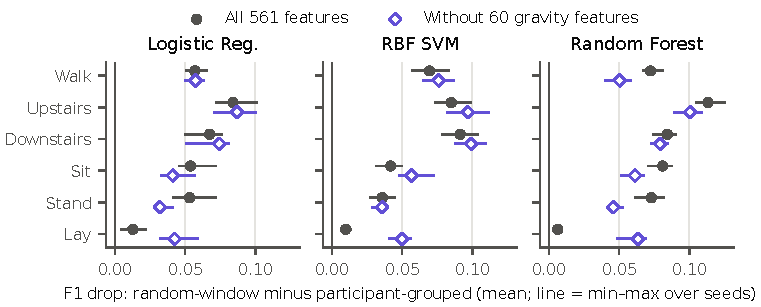
\includegraphics[width=\linewidth]{figures/per_class_drop_ablation.pdf}
\caption{Per-class F1 drop, random-window minus participant-grouped CV, with and without gravity features.}
\label{fig:ablation}
\end{figure}

\textbf{Which activities carry the gap (RQ3)?} In Fig.~\ref{fig:ablation} (filled markers), the walking classes drop for every model, walking upstairs most (LR \NdropLRUpstairs, SVM \NdropSVMUpstairs, RF \NdropRFUpstairs). Laying barely changes (at most \NdropLRLay); sitting and standing drop by \NdropSVMStand--\NdropRFSit.

\textbf{Does the gravity family explain the static-posture gap?} Only partly, and not for every model. Without it, participant-grouped macro-F1 falls for all models (LR \NablLRMacroPfull{}\,$\to$\,\NablLRMacroPng, SVM \NablSVMMacroPfull{}\,$\to$\,\NablSVMMacroPng, RF \NablRFMacroPfull{}\,$\to$\,\NablRFMacroPng), but the overall gap does not shrink (LR \NablLRMacrofull{}\,$\to$\,\NablLRMacrong, RF \NablRFMacrofull{}\,$\to$\,\NablRFMacrong, SVM \NablSVMMacrofull{}\,$\to$\,\NablSVMMacrong). For LR and RF the sitting and standing gaps shrink (LR sit \NablLRSitfull{}\,$\to$\,\NablLRSitng{} in \NablLRSitn{} of \Nnseeds{} seeds; RF stand \NablRFStandfull{}\,$\to$\,\NablRFStandng{} in \NablRFStandn), but mainly because random-window scores fall more (LR random-window sit F1 \NablLRSitRfull{}\,$\to$\,\NablLRSitRng); for the SVM the sitting gap grows. The laying gap grows for all models (LR \NablLRLayfull{}\,$\to$\,\NablLRLayng), since without orientation laying is no longer trivially separable. Permuting the family in held-out folds lowers grouped macro-F1 from \NpermLRbase{} to \NpermLR{} (LR) and \NpermRFbase{} to \NpermRF{} (RF). The gravity features are therefore heavily used and mostly transferable, with some participant-specific information for sitting and standing in LR and RF; we did not test whether body geometry or posture causes this.

\textbf{Model selection and test.} The best grouped-CV scores were \NtuneLR{} for LR ($C{=}\NtuneLRC$), \NtuneSVM{} for the SVM ($C{=}\NtuneSVMC$, $\gamma{=}\NtuneSVMgamma$) and \NtuneRF{} for RF (\NtuneRFtrees{} trees, \NtuneRFmf{} features, leaf \NtuneRFleaf, at the grid edge but within 0.002 of its neighbours). The \Nselmodel{} was selected (\Nselcv{}\,$\pm$\,\Nselcvsd{} over folds), only \Nselmargin{} ahead of LR, far less than the fold SD: a narrow preference, not reliable superiority. Refitted on all training windows, it reaches macro-F1 \Ntestf, accuracy \Ntestacc{} and BA \Ntestbal{} on the nine test participants (Fig.~\ref{fig:test}); these are close but not identical because test class shares lie between \Ntestsharemin\% and \Ntestsharemax\%. This is \Ntestminuscv{} from its grouped-CV estimate and below random-window CV of the fixed SVM (\NmfSVMR); with nine people it is a single noisy draw (grouped fold SD $\approx$\,\NfsdSVMP), and per-participant macro-F1 ranges from \Nsubjmin{} to \Nsubjmax{} (median \Nsubjmed). The main errors are sitting predicted as standing (\NconfAn{} windows, \NconfApct\%), downstairs as upstairs (\NconfBn) and upstairs as walking (\NconfCn); only \Nncross{} of \Nnerr{} errors cross between static and moving activities.

\begin{figure}[t]
\centering
\begin{minipage}[c]{0.40\linewidth}
\centering
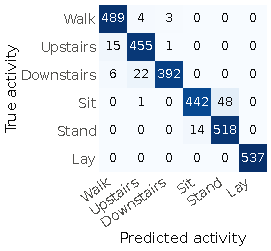
\includegraphics{figures/test_confusion_matrix.pdf}
\end{minipage}\hfill
\begin{minipage}[c]{0.52\linewidth}
\centering\footnotesize
\begin{tabular}{lccc}
\toprule
Class & Prec. & Rec. & F1 \\
\midrule
Walk & \NtestprecWalk & \NtestrecWalk & \NtestfoneWalk \\
Upstairs & \NtestprecUpstairs & \NtestrecUpstairs & \NtestfoneUpstairs \\
Downstairs & \NtestprecDownstairs & \NtestrecDownstairs & \NtestfoneDownstairs \\
Sit & \NtestprecSit & \NtestrecSit & \NtestfoneSit \\
Stand & \NtestprecStand & \NtestrecStand & \NtestfoneStand \\
Lay & \NtestprecLay & \NtestrecLay & \NtestfoneLay \\
\midrule
Macro-F1 / Acc. / BA & \multicolumn{3}{c}{\Ntestf{} / \Ntestacc{} / \Ntestbal} \\
\bottomrule
\end{tabular}
\end{minipage}
\caption{Selected \Nselmodel{} on the official test set (2,947 windows, 9 participants): confusion matrix (counts; shading = row \%) and per-class scores.}
\label{fig:test}
\end{figure}

\section{Limitations and Conclusion}
With 30 people (21 for development), grouped folds hold four or five people and all spreads are descriptive. Activities were scripted in a laboratory with one waist-worn phone, and we use only the supplied features. Segment grouping does not remove correlation between nearby non-overlapping windows. Tuning used one grouped split of the same people, and we did not run leave-one-subject-out CV. \emph{Conclusion.} On UCI HAR, random-window CV overestimates macro-F1 on unseen participants by \Ngapmodelmin--\Ngapmodelmax{} in every split, through shared participants and shared samples, and understates fold-to-fold variability; new-user models need participant-grouped validation.

\section{Reproducibility, Test-Set Access and AI Use}
\label{sec:repro}
\textbf{Code:} [REPOSITORY URL]. \texttt{scripts/run\_all.sh} downloads the data and runs every development step on the training partition; \texttt{scripts/run\_final\_test.sh} is the separate test stage, which records SHA-256 hashes of the code and the selection before scoring. Development ran on Kaggle CPU kernels (\Nncpu{} vCPUs, Python \Npyver, scikit-learn \Nsklearn).
\textbf{Test-set access.} The official test partition has been scored three times. A local pipeline smoke test scored LR, $C{=}\NsmokeC$ (macro-F1 \Nsmoketestf); the first full run scored LR, $C{=}\NrunoneC$ (\Nrunonetestf); this revision scored the \Nselmodel{} above once. Code, grids and models did not change between the first two; the revision's changes follow reviewer requests, not test scores. As earlier scores were seen, the holdout is not fully unseen, so we report it as a supplementary check.
\textbf{AI use:} Claude Code (Anthropic, Claude Opus 5.5) wrote the code, ran the experiments, made the figures and drafted this paper from the student's brief and the reviewers' revision instructions. [STUDENT: state truthfully which code, results and claims you inspected, reran, corrected or rewrote yourself.]

{\small\setlength{\bibsep}{2pt}
\begin{thebibliography}{6}
\bibitem[Anguita et~al.(2013)]{anguita2013}
D.~Anguita, A.~Ghio, L.~Oneto, X.~Parra, and J.~L. Reyes-Ortiz.
\newblock A public domain dataset for human activity recognition using smartphones.
\newblock In \emph{Proc.\ ESANN}, pages 437--442, 2013.

\bibitem[Bragan{\c{c}}a et~al.(2022)]{braganca2022}
H.~Bragan{\c{c}}a, J.~G. Colonna, H.~A.~B.~F. Oliveira, and E.~Souto.
\newblock How validation methodology influences human activity recognition mobile systems.
\newblock \emph{Sensors}, 22(6):2360, 2022. doi:\nolinkurl{10.3390/s22062360}.

\bibitem[Pedregosa et~al.(2011)]{sklearn}
F.~Pedregosa, G.~Varoquaux, A.~Gramfort, V.~Michel, B.~Thirion, et~al.
\newblock Scikit-learn: Machine learning in {P}ython.
\newblock \emph{Journal of Machine Learning Research}, 12:2825--2830, 2011.

\bibitem[Rehman et~al.(2024)]{rehman2024}
S.~U. Rehman, A.~Ali, A.~M. Khan, and C.~Okpala.
\newblock Human activity recognition: A comparative study of validation methods and impact of feature extraction in wearable sensors.
\newblock \emph{Algorithms}, 17(12):556, 2024. doi:\nolinkurl{10.3390/a17120556}.

\bibitem[Reyes-Ortiz et~al.(2013)]{uci_har}
J.~Reyes-Ortiz, D.~Anguita, A.~Ghio, L.~Oneto, and X.~Parra.
\newblock Human activity recognition using smartphones.
\newblock UCI Machine Learning Repository, 2013. doi:\nolinkurl{10.24432/C54S4K}.

\bibitem[Saeb et~al.(2017)]{saeb2017}
S.~Saeb, L.~Lonini, A.~Jayaraman, D.~C. Mohr, and K.~P. Kording.
\newblock The need to approximate the use-case in clinical machine learning.
\newblock \emph{GigaScience}, 6(5):gix019, 2017. doi:\nolinkurl{10.1093/gigascience/gix019}.
\end{thebibliography}
}

\end{document}
